%File: formatting-instruction.tex
\documentclass[letterpaper]{article}
\usepackage{aaai}
\usepackage{times}
\usepackage{helvet}
\usepackage{courier}
\usepackage{amsmath}
\usepackage{amsfonts}
\usepackage{graphicx}
\usepackage{hyperref}
\usepackage{xcolor}

\frenchspacing
\setlength{\pdfpagewidth}{8.5in}
\setlength{\pdfpageheight}{11in}
\pdfinfo{
/Title (Continuous Control Project Report)
/Author (Piero Macaluso)}
\setcounter{secnumdepth}{0}  
 \begin{document}
% The file aaai.sty is the style file for AAAI Press 
% proceedings, working notes, and technical reports.
%
\title{Continuous Control Project Report}
\author{Piero Macaluso}
\maketitle

\section{Introduction}

The purpose of this document is to briefly present the work done in this project, along with the algorithm used and implemented, but also with a showcase of the results obtained.

This document can be divided into 4 parts:

\begin{itemize}
\item \textbf{Introduction}: the current section;
\item \textbf{Learning Algorithm}: an overview of the approaches and methods used to solve the problem;
\item \textbf{Results}: a presentation of the results reached with plots and GIFs of the best episodes;
\item \textbf{Future Work}: some ideas on how to improve the actual algorithm.
\end{itemize}

\section{Learning Algorithms}

The environment selected for this project consists of the second option proposed, the one with 20 agents that interacts simultaneously with the environment.

The chosen algorithm was the Deep Deterministic Policy Gradient (DDPG) one \cite{lillicrap2015continuous}. This algorithms roots from the adaptation of the ideas underlying the success of Deep Q-Learning to make it compatible to situation that requests a continuous action space. It is an actor-critic, model-free algorithm based on the deterministic policy gradient.

DDPG algorithm exploits 4 neural networks: the local actor $\pi$, the local critic $Q$, the target actor $\pi'$ and the target critic $Q'$.
In the context of DDPG, the Bellman equation is the starting point for learning an approximator to $Q^*(s,a)$ of Q-Learning.
The approximator is parametrised by $\phi$ and the value network is updated and optimised by minimising the loss defined in Equation \ref{eq:ddpgloss} where $d_t$ is a flag which indicates whether the  state $s_{t+1}$ is terminal.
\begin{equation}\label{eq:ddpgloss}
	\begin{gathered}
		L(\phi) = \mathbb{E}_{s_t\sim \rho^\beta, a_t\sim \beta,r_t\sim E}[(Q(s_t, a_t|\phi)-y_t)^2] \\
		y_t = r(s_t, a_t) + \gamma (1-d_t)Q'(s_{t+1}, \pi'(s_t+1|\bar{\theta})|\bar{\phi})
	\end{gathered}
\end{equation}
It is clear from Equation \ref{eq:ddpgloss} that the loss is calculated starting from the transitions generated by the policy $\beta$, which consists in experiences sampled from a \textit{replay buffer}. This step is essential to make the data gathered from experiences independent and identically distributed (i.i.d.).

From the policy perspective, the objective is to maximise Equation \ref{eq:expected} calculating the policy loss through the derivative of the objective function concerning the policy parameter Equation \ref{eq:derivative_exp}.
However, since the algorithm is updating the policy in an off-policy way with batches of experience, it is possible to use the mean of the sum of gradients calculated from the mini-batch Equation \ref{eq:mean_gradient}.

\begin{equation}\label{eq:expected}
	J(\theta) = \mathbb{E}[Q(s,a)|_{s=s_t,a=\pi(s_t)}]
\end{equation}
\begin{equation}\label{eq:derivative_exp}
	\nabla_{\theta} J(\theta) \approx \nabla_a Q(s,a) \nabla_{\theta}\pi(s|\theta)
\end{equation}
\begin{equation}\label{eq:mean_gradient}
	\nabla_{\theta} J(\theta) \approx \frac{1}{N}\sum_{i}\big[\nabla_a Q(s,a| \phi)|_{s=s_i, a = \pi(s_i)} \nabla_{\theta}\pi(s|\theta)|_{s=s_i}\big]
\end{equation}

\subsection{Hyper-parameters}

The environment state and action space is very simple and it does not require convolutional neural networks. For this reason, both the actor and the critic were implemented with 2 fully connected layer with 128 neurons as hidden size. Both networks exploits \textit{Rectified Linear Unit} (ReLU) as non-linearity for each layer. The policy uses Tanh as non-linearity for the last layer, while the critic does not use non-linearity for the last layer. The hyper-parameters used are presented in Table \ref{table:hp}.

Before reaching the solution of the problem, we needed to try and fail a lot of times. We added to the algorithm \textit{gradient clipping} for the critic and \textit{weight initialization} for both networks. Initially we used Batch Normalization for each layer, but this lead the agent to reach a maximum and then fall back to lower rewards. The removal of this feature was crucial in the resolution of the problem.

For what conserns the noise, we decided to implement a degradation of the $\sigma$ parameter until a minimum of $0.01$ with a noise decay equal to $0.96$.

\begin{table}[]
\begin{tabular}{rl}
\textbf{Hyper-parameters}    & \textbf{Value}        \\
Memory Buffer Size          & $10^6$ \\
Batch Size                  & $128$                    \\
Gamma                       & $0.99$                  \\
Tau                         & $10^{-3}$                 \\
Learning Rate               & $1\times 10^{-3}$                  \\
Learning Frequency          & $10$ updates every $20$ steps            \\
Target Update Frequency        & every $10$ learning steps            \\

Ornstein-Uhnlebeck Noise &  $\theta=0.15$, $\sigma=0.20$ decaying
\end{tabular}
\caption{Hyper-parameters used in the training process}
\label{table:hp}
\end{table}

\section{Results}

The number of episodes to play was fixed at $500$, however, the agent took just $103$ episodes to reach an average score on all 20 agents on the last 100 episodes greater than $30.0$. We decided to cut the training process at $150$ episodes. The highest average score on the last 100 episodes was equal to $36.69$ reached in $131$ episodes.

To find the best solution, a test phase of 10 episodes was implemented and started every 50 training episodes to evaluate the results without taking into account exploration noise. As shown in Figure \ref{fig:plot}, the best test result was found at episode $150$ \footnote{GIF reporting a handful of seconds of the testing phase \href{https://github.com/pieromacaluso/continuous-control/blob/17becf554171be594d56cea02d1f0855339915f8/stuff/solved_gif.gif}{\textcolor{blue}{here}}} with an average of $39.29$ over 10 episodes.

\begin{figure}[]
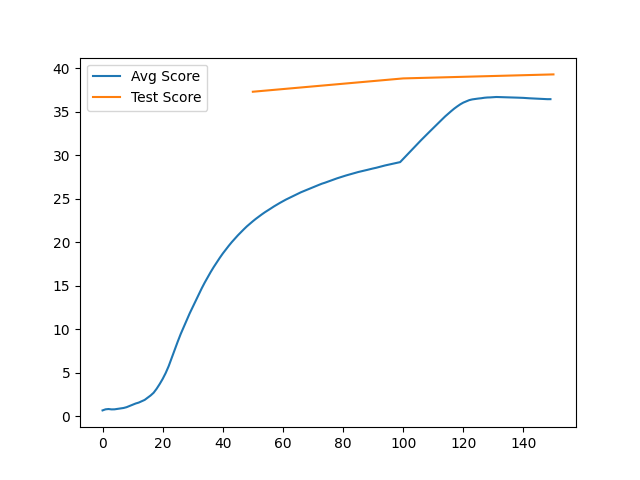
\includegraphics[width=\linewidth]{img/avg.png}
\caption{Training and Test Scores History\label{fig:plot}}
\end{figure}   

\begin{figure}[]
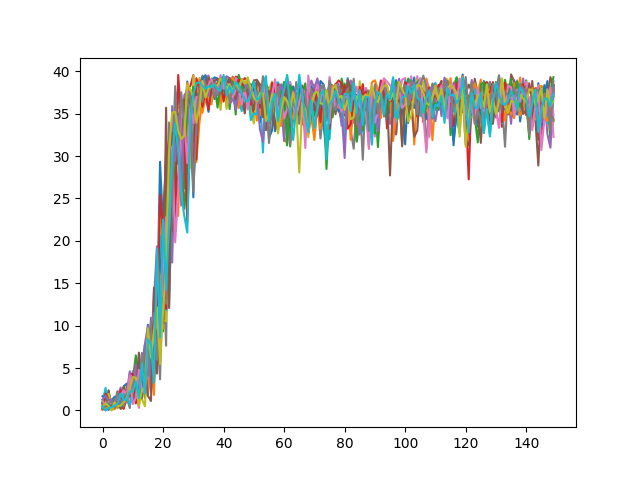
\includegraphics[width=\linewidth]{img/scores.png}
\caption{Training Scores of all 20 agents\label{fig:plot2}}
\end{figure}   

\section{Future Work}

The results obtained were very encouraging and positive. Despite this, there are a lot of further improvement that goes beyond the DDPG algorithm implemented in this project. Insights about this topic can be found in the D4PG \cite{barth2018distributed} and Noisy Layers instead of Action Noise \cite{fortunato2017noisy}.


\bibliographystyle{aaai}
\bibliography{bibliography}
\end{document}